\section{Lineare Abtastregelungen}


\subsection{Allgemeines}

Abtastregelungssysteme entstehen, wenn in einen kontinuierlich arbeitenden Regelkreis ein oder mehrere Glieder eingefügt werden, die Größen nicht kontinuierlich, sondern nur zu diskreten Zeitpunkten übertragen.
Der häufigste Fall ist der der Übertragung zu äquidistanten Zeitpunkten; er soll im Folgenden ausschließlich betrachtet werden.

Die zeitdiskrete Übertragung von Größen kann notwendig werden, weil
\begin{enumerate}[label=\alph*)]
	\item die Regelgröße nicht kontinuierlich messbar ist,
	\item die Stellgröße nur zu bestimmten Zeitpunkten geändert werden kann,
	\item die Regeleinrichtung nur zeitdiskrete Größen verarbeiten kann.
\end{enumerate}
Einige Beispiele sind
\begin{enumerate}[label=\alph*)]
	\item Analysegeräte, die diskontinuierlich arbeiten;

	Prozesse, denen nur zu bestimmten Zeiten Proben entnommen werden können (z.B. Hochofen beim Abstrich);
	\item Thyristorstellglieder für Gleichstrommotoren, die nur im Takt der Wechselspannung arbeiten können;
	\item\label{enum:6-1:2-c} digitale, zeitdiskret arbeitende Regler (z.B. Regler auf der Grundlage von Mikrorechnern);

	Prozessrechner, die unter Umständen mehrere (10 bis 200) Regelkreise bedienen.
\end{enumerate}
Der unter c) aufgeführte Fall der direkten Steuerung und Regelung durch einen Rechner (auch DDC, \underline{d}irect \underline{d}igital, \underline{c}ontrol genannt) soll hier bevorzugt behandelt werden, obgleich die gewonnenen Hilfsmittel ohne Schwierigkeiten auch auf die anderen Fälle anzuwenden sind.
Ein Regelkreis mit kontinuierlich arbeitender Regelstrecke und abtastend arbeitendem Regler kann durch die im Bild \ref{fig:6-1} wiedergegebene Struktur dargestellt werden.
Auch wenn der Regler durch einen Prozessrechner verwirklicht wird, der über Eingabesammler (Messstellenumschalter) und Ausgabeverteiler zeitlich nacheinander mit einer größeren Zahl von (Teil-)Regelstrecken verbunden wird, so führt die Betrachtung nur eines Regelkreises auf die Struktur von Bild \ref{fig:6-1}.
Sie soll für die folgenden Betrachtungen zugrunde gelegt werden.
\begin{figure}[ht]
	\centering
	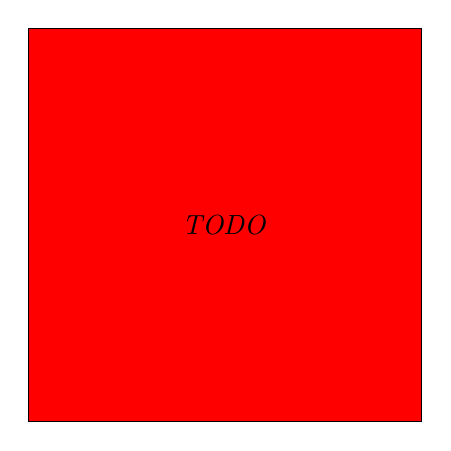
\begin{tikzpicture}
		\filldraw[fill=red] (0,0) rectangle (5,5) node[pos=.5] {\emph{TODO}};
 	\end{tikzpicture}
	\caption{Einfache Abtastungsregelung}
	\label{fig:6-1}
\end{figure}
Die zeitliche Diskretisierung kontinuierlicher Größen, im Folgenden Abtastung genannt, kann man so deuten, dass der kontinuierlichen Größe \(e\parentheses*{t}\) entweder eine Folge äquidistanter Impulse \(e^*\parentheses*{t}\) oder eine Folge von Werten \(e_k\) zugeordnet wird (Bild \ref{fig:6-2}).
Die Flächen der Impulse entsprechen dabei den zugehörigen Werten der kontinuierlichen Größe.
Ihr zeitlicher Abstand ist das Arbeitsintervall \(T\).
\begin{figure}[ht]
	\centering
	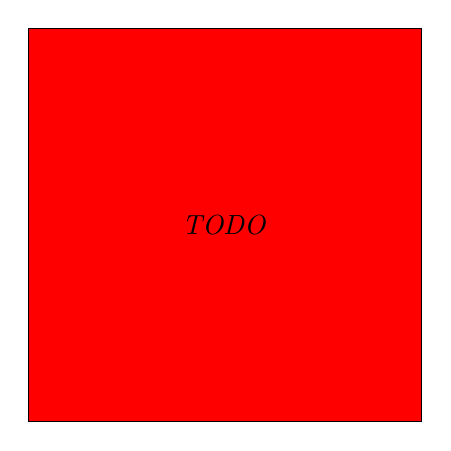
\begin{tikzpicture}
		\filldraw[fill=red] (0,0) rectangle (5,5) node[pos=.5] {\emph{TODO}};
 	\end{tikzpicture}
	\caption{Abtaster}
	\label{fig:6-2}
\end{figure}
Die zeitdiskrete Größe \(e^*\parentheses*{t}\) bzw. die Wertefolge \(e_k\) kann von zeitdiskret arbeitenden Übertragungsgliedern weiterverarbeitet werden.
Diese Übertragungsglieder können als impulsübertragende Systeme behandelt werden, die eine Eingangs-Impulsfolge \(e^*\parentheses*{t}\) in eine Ausgangs-Impulsfolge \(y^*\parentheses*{t}\) umformen oder als Systeme, die aus einer Eingangs-Wertefolge \(e_k\) eine Ausgangs-Wertefolge \(y_k\) erzeugen (Bild \ref{fig:6-3}).
Eingangs- und Ausgangsfolgen haben das gleiche Abtastintervall \(T\).
Meist werden die zeitdiskreten Übertragungssysteme so definiert, dass alle Glieder eines Regelkreises mit dem gleichen festen Zeitraster arbeiten.
Dies entspricht häufig nicht völlig der Wirklichkeit, vereinfacht aber manche Betrachtungen erheblich.
\begin{figure}[ht]
	\centering
	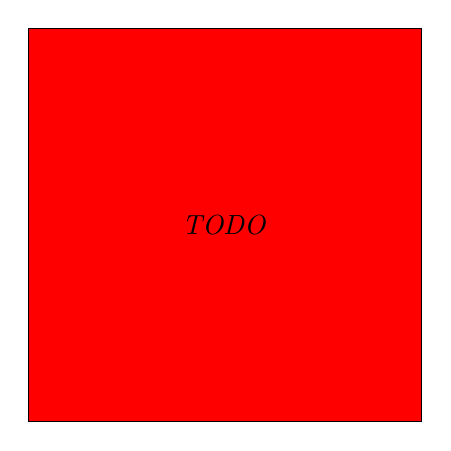
\begin{tikzpicture}
		\filldraw[fill=red] (0,0) rectangle (5,5) node[pos=.5] {\emph{TODO}};
 	\end{tikzpicture}
	\caption{Zeitdiskretes Übertragungsglied (Regler)}
	\label{fig:6-3}
\end{figure}
Zur Umwandlung zeitdiskreter impulsförmiger Größen oder von Wertefolgen in kontinuierliche Funktionen, wie sie als Eingangsgrößen kontinuierlich arbeitender Systeme erforderlich sind, dienen so genannte Halteglieder (Bild \ref{fig:6-4}).
Das einfachste und in den meisten Fällen benutzte Halteglied 0. Ordnung erzeugt aus einem Eingangswert eine Ausgangsgröße entsprechender Amplitude und hält diese bis zum Eintreffen des nächsten Eingangswertes konstant.
Halteglieder für Impulsfolgen arbeiten in analoger Weise.
\begin{figure}[ht]
	\centering
	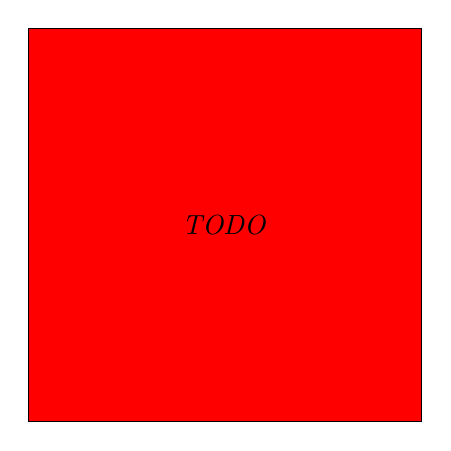
\begin{tikzpicture}
		\filldraw[fill=red] (0,0) rectangle (5,5) node[pos=.5] {\emph{TODO}};
 	\end{tikzpicture}
	\caption{Halteglied 0. Ordnung}
	\label{fig:6-4}
\end{figure}
Aus Bild \ref{fig:6-5} ist zu erkennen, dass Abtaster und Halteglied zusammen mit einem verzögerungsfreien zeitdiskreten Übertragungsgleid ungefähr wie ein Glied mit einer Totzeit von \(\frac{T}{2}\) wirken.
D.h. durch die Umwandlung einer kontinuierlichen in eine zeitdiskrete Größe und die nachfolgende Rückumsetzung in eine kontinuierliche wird die Größe um etwa \(\frac{T}{2}\) verzögert.
Dies hat u.a. zur Folge, dass die Stabilitätseigenschaften von Regelkreisen mit abtastend arbeitenden Reglern schlechter sind als die von Regelkreisen mit kontinuierlich arbeitenden Reglern.
\begin{figure}[ht]
	\centering
	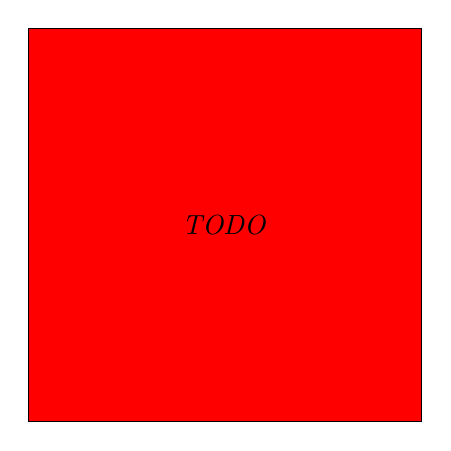
\begin{tikzpicture}
		\filldraw[fill=red] (0,0) rectangle (5,5) node[pos=.5] {\emph{TODO}};
 	\end{tikzpicture}
	\caption{Abtaster mit Halteglied und Größenverläufe}
	\label{fig:6-5}
\end{figure}
Mit Überlegungen, die hier nicht wiedergegeben werden sollen, gewinnt man zur angenäherten Beschreibung des aus Abtaster und Halteglied bestehenden Teilsystems den Frequenzgang
\begin{equation}
	G_{AH}\parentheses*{j\omega} = \frac{1 - e^{-j\omega T}}{j\omega T} = \frac{\sin\frac{\omega T}{2}}{\frac{\omega T}{2}} \cdot e^{-j\frac{\omega T}{2}}.
\end{equation}
Für Frequenzen bis etwa \(\omega T = 1\) weicht der Betrag des Frequenzganges um weniger als \(5\%\) von Eins ab, sodass die eingeführte Näherung durch ein Totzeitglied mit einer Totzeit von \(\frac{T}{2}\) für niedrige Frequenzen und/oder kleine Abtastintervalle ausreicht.

Beim Entwurf einer direkten digitalen Regelung hat man i. Allg. ein System nach Bild \ref{fig:6-1} zu behandeln, das aus einer kontinuierlichen Regelstrecke und einem zeitdiskreten Regler besteht.
Das resultierende Gesamtsystem kann man entweder als zeitdiskretes oder als kontinuierliches System beschreiben.
Entscheidet man sich für das letztere Vorgehen, so muss man das aus Abtaster, Regler und Halteglied bestehende Teilsystem durch einen äquivalenten Frequenzgang oder eine Übertragungsfunktion beschreiben.
Im anderen Fall muss man Halteglied, Regelstrecke und Abtaster durch eine zeitdiskrete Übertragungsfunktion oder eine Differenzengleichung beschreiben und die kontinuierliche Führungs- und Störgröße durch zeitdiskrete Größen ersetzen.

Ohne auf Einzelheiten einzugehen kann man sagen, dass die Darstellung des Gesamtsystems als kontinuierliches System dann zweckmäßig sein wird, wenn das Abtastintervall \(T\) so klein ist in Relation zur Dynamik des Systems, dass der Abtastvorgang das Gesamtverhalten nicht wesentlich beeinflusst.
In solchen Fällen kann es genügen, Abtaster und Halteglied durch ein Glied mit einer Totzeit \(\frac{T}{2}\) zu ersetzen, das dann der Regelstrecke zugerechnet wird, einen für diese Regelstrecke geeigneten kontinuierlichen Regler zu spezifizieren und diesem dann einen zeitdiskreten Regelalgorithmus zuzuordnen.
Einzelheiten werden im folgenden Abschnitt \ref{sec:6-2} behandelt.

Wenn das Abtastintervall in Relation zur Dynamik des Systems nicht mehr vernachlässigbar klein ist, wird man i. Allg. zweckmäßigerweise eine Beschreibung des Gesamtsystems als zeitdiskretes System anstreben.
Dazu benötigt man die zeitdiskrete Darstellung des Teilsystems bestehend aus Halteglied, Regelstrecke und Abtaster und hat diese mit der Darstellung des zeitdiskreten Reglers zu verbinden.
Dazu notwendige Verfahren werden in dieser Vorlesung aber nicht behandelt.


\subsection{Lineare zeitdiskrete Übertragungssysteme}\label{sec:6-2}

Der Regler in Bild \ref{fig:6-1} ist ein lineares, zeitdiskretes Übertragungsglied.
Allgemein wandeln solche Übertragungsglieder eine Folge von Eingangswerten \(u_k\) oder Eingangsimpulsen \(u^*\parentheses*{t}\) in eine Folge von Ausgangswerten \(y_k\) oder Ausgangsimpulsen \(y^*\parentheses*{t}\) um.

In Analogie zur Beschreibung linearer kontinuierlicher Übertragungssysteme durch lineare Differentialgleichungen können zeitdiskrete Übertragungssysteme durch Differenzengleichungen beschrieben werden.
Solche Differenzengleichungen für Wertefolgen sind von der Form
\begin{equation}\label{eq:6-2}
	a_0 y_k + a_1 y_{k - 1} + \cdots + a_n y_{k - n} = b_0 u_k + b_1 u_{k - 1} + \cdots + b_m u_{k - m}
\end{equation}
mit \(\parentheses*{u_k}\) als Folge der Eingangswerte und \(\parentheses*{y_k}\) als Folge der Ausgangswerte.
Gleichung \eqref{eq:6-2} lässt sich kurz als
\begin{equation}\label{eq:6-3}
	\sum_{i = 0}^n a_i y_{k - i} = \sum_{i = 0}^m b_i u_{k - i}
\end{equation}
schreiben und nach dem Wert der Ausgangsfolge zum Zeitpunkt \(k\) auflösen
\begin{align}
	\begin{split}
		y_k &= \frac{1}{a_0}\parentheses*{b_0 u_k + b_1 u_{k - 1} + \cdots + b_m u_{k - m} - a_1 y_{k - 1} - \cdots - a_n y_{k - n}}\\
		&= \frac{1}{a_0}\parentheses*{\sum_{i = 0}^m b_i u_{k - i} - \sum_{i = 1}^n a_i y_{k - i}}.
	\end{split}
\end{align}
Differenzengleichungen, die für kleine Abtastintervalle \(T\) die Differenziation oder Integration kontinuierlicher Größen ausreichend genau annähern, kann man leicht gewinnen.
So lässt sich die erste Ableitung
\begin{equation}\label{eq:6-5}
	y\parentheses*{t} = K_D \cdot \dot{u}\parentheses*{t}
\end{equation}
durch einen Differenzenquotienten annähern.
Zweckmäßigerweise benutzt man dabei die sog. Rückwärtsdifferenz, weil diese keine Werte aus der Zukunft erfordert und erhält als zeitdiskretes Äquivalent zu Gleichung \eqref{eq:6-5}
\begin{equation}\label{eq:6-6}
	y_k = \frac{K_D}{T}\parentheses*{u_k - u_{k - 1}}.
\end{equation}
Um die Integration
\begin{equation}
	y\parentheses*{t} = K_I \int_0^t u\parentheses*{\tau}\d\tau
\end{equation}
anzunähern, bedient man sich der Rechteckregel und erhält
\begin{equation}
	y_k = K_I \cdot T \cdot \sum_{i = 1}^k u_i = y_{k - 1} + K_I \cdot T \cdot u_k
\end{equation}
oder
\begin{equation}
	y_k - y_{k - 1} = K_I \cdot T \cdot u_k.
\end{equation}
Mit Hilfe der Gleichung \eqref{eq:6-5} und \eqref{eq:6-6} lässt sich die Differentialgleichung eines Verzögerungsgliedes 1. Ordnung
\begin{equation}\label{eq:6-10}
	T_S \dot{y} + y = K \cdot u
\end{equation}
umformen in die näherungsweise äquivalente Differenzengleichung
\begin{equation}
	\frac{T_S}{T}\parentheses*{y_k - y_{k - 1}} + y_k = K \cdot u_k.
\end{equation}
Durch Umordnen
\begin{equation}\label{eq:6-12}
	\parentheses*{\frac{T_S}{T} + 1}y_k - \frac{T_S}{T}y_{k - 1} = K \cdot u_k
\end{equation}
erhält man eine Differenzengleichung analog der Form in Gleichung \eqref{eq:6-2}.

Unter der Voraussetzung, dass eine gegebene Differenzengleichung
\begin{equation}
	a_0 y_k + a_1 y_{k - 1} = b_0 u_k
\end{equation}
durch die Anwendung der Rückwärtsdifferenzen auf eine Differentialgleichung gemäß Gleichung \eqref{eq:6-10} entstanden ist, können durch Koeffizientenvergleich mit Gleichung \eqref{eq:6-12} und bei gegebenen \(a_0\), \(a_1\) und \(b_0\) die Parameter \(T_S\) und \(K\) des kontinuierlichen Systems bestimmt werden.
Es gilt dann
\begin{equation}
	T_S = \parentheses*{a_0 - 1 \cdot T} = -a_1 \cdot T, \quad K = b_0, \quad a_0 + a_1 = 1.
\end{equation}
Bei der Behandlung von totzeitbehafteten Systemen beschränkt man sich üblicherweise auf den Fall, dass sich die Totzeit als Vielfaches des Abtastintervalls \(T\) darstellen lässt.
Das \(PT_t\)-Glied
\begin{equation}
	y\parentheses*{t} = K \cdot u\parentheses*{t - T_t}
\end{equation}
wird daher mit \(T_t = d \cdot T\) durch die Differenzengleichung
\begin{equation}
	y_k = K \cdot u_{k - d}
\end{equation}
beschrieben.

Der statische Übertragungsfaktor \(K\) eines stabilen zeitdiskreten Übertragungssystems lässt sich aus der Differenzengleichung leicht gewinnen, wenn man bedenkt, dass für die Eingangsfolge
\begin{equation}
	\parentheses*{u_k} = \parentheses*{1, 1, 1, \ldots}
\end{equation}
im eingeschwungenen Zustand die Ausgangsgröße
\begin{equation}
	y_k = K \quad \forall k
\end{equation}
sein muss.
Einsetzen in Gleichung \eqref{eq:6-3} ergibt
\begin{equation}
	\sum_{i = 0}^n a_i \cdot K = \sum_{i = 0}^m b_i \cdot 1
\end{equation}
und damit das Ergebnis
\begin{equation}
	K = \frac{\sum_{i = 0}^m b_i}{\sum_{i = 0}^n a_i}.
\end{equation}
Zeitdiskreten Übertragungssystemen lässt sich ein Frequenzgang zuordnen, der die Übertragung (abgetasteter) harmonischer Funktionen beschreibt.
Wenn in Analogie zum Vorgehen im Abschnitt 3.9 (Frequenzgang und Differentialgleichung) die Übertragung einer komplexen harmonischen Eingangsgröße
\begin{equation}
	\underline{u}\parentheses*{t} = \underline{u}\parentheses*{\cos\omega t + j\sin\omega t} = \underline{u}e^{j\omega t}
\end{equation}
mit dem Zeiger \(\underline{u}\) zur Darstellung von Amplitude und Phasenwinkel betrachtet wird, so ist die zugehörige komplexe Eingangswertefolge
\begin{equation}
	\underline{u}_k = \underline{u}e^{j\omega kT}.
\end{equation}
Die resultierende komplexe Ausgangswertefolge wird nun genauso konstruiert, d.h. man nimmt an, dass sie durch Abtasten einer kontinuierlichen harmonischen Funktion
\begin{equation}
	\underline{y}\parentheses*{t} = \underline{y}e^{j\omega t}
\end{equation}
entsteht.
Man erhält
\begin{equation}
	\underline{y}K = \underline{y}e^{j\omega kT}.
\end{equation}
Jetzt ist zu prüfen, ob die beiden komplexen Wertefolgen die Differenzengleichung \eqref{eq:6-2} erfüllen.
Einsetzen ergibt
\begin{equation}
	\underline{y}\brackets*{a_0 e^{j\omega kT} + a_1 e {j\omega\parentheses*{k - 1}T} + \cdots + a_n e^{j\omega\parentheses*{k - n}T}} = \underline{u}\brackets*{b_0 e^{j\omega kT} + b_1 e^{j\omega\parentheses*{k - 1}T} + \cdots + b_m e^{j\omega\parentheses*{k - m}T}}.
\end{equation}
Im Blick auf die Ableitung des Frequenzgangs aus der Differentialgleichung für kontinuierliche Systeme liegt es nahe, den Quotienten der beiden Zeiger zu bilden und dabei den Ausdruck \(e^{j\omega kT}\) zu kürzen.
Das Ergebnis
\begin{equation}
	\frac{\underline{y}}{\underline{u}} = \frac{b_0 e^{j\omega T \cdot 0} + b_1 e^{j\omega T \cdot \parentheses*{-1}} + \cdots + b_m e^{j\omega T \cdot \parentheses*{-m}}}{a_0 e^{j\omega T \cdot 0} + a_1 e^{j\omega T \cdot \parentheses*{-1}} + \cdots + a_m e^{j\omega T \cdot \parentheses*{-n}}}
\end{equation}
entspricht der später zu behandelnden \(z\)-Übertragungsfunktion, wenn man \(z = e^{j\omega T}\) setzt.
Hier gilt
\begin{equation}
	\frac{\underline{y}}{\underline{u}} = G\parentheses*{e^{j\omega T}} = \frac{b_0 + b_1 e^{-j\omega T} + b_2 e^{-2j\omega T} + \cdots + b_m e^{-mj\omega T}}{a_0 + a_1 e^{-j\omega T} + a_2 e^{-2j\omega T} + \cdots + a_m e^{-nj\omega T}}
\end{equation}
und dies ist der ``Frequenzgang des zeitdiskreten Übertragungssystems''.
Der Frequenzgang hat nicht die Kreisfrequenz als Argument sondern eine Exponentialfunktion mit imaginärem Exponenten.
Solche Exponentialfunktionen sind periodisch in \(2\pi\) und daher ist der Frequenzgang selbst periodisch in \(\frac{2\pi}{T}\).
Die Konsequenzen sollen an zwei Beispielen erläutert werden.

Ein zeitdiskretes Differenzierglied hat die Differenzengleichung
\begin{equation}
	y_k = \frac{K_D}{T}\parentheses*{u_k - u_{k - 1}}
\end{equation}
und den zugehörigen Frequenzgang
\begin{equation}
	G_D\parentheses*{e^{j\omega T}} = \frac{K_D}{T}\parentheses*{1 - e^{-j\omega T}}.
\end{equation}
Die Ortskurve dieses Frequenzgangs hat für \(\frac{K_D}{T} = 1\) die Form eines Kreises mit dem Radius \(1\) und dem Mittelpunkt \(1\) (Bild \ref{fig:6-6}).
\begin{figure}[ht]
	\centering
	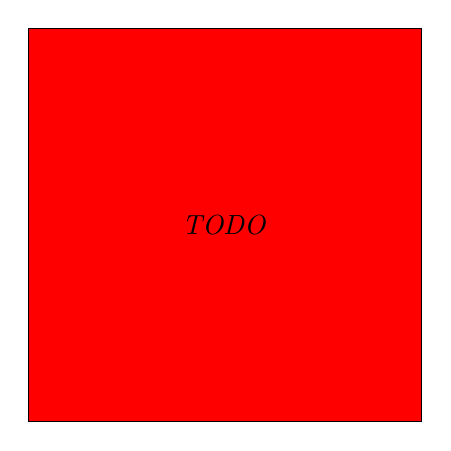
\begin{tikzpicture}
		\filldraw[fill=red] (0,0) rectangle (5,5) node[pos=.5] {\emph{TODO}};
 	\end{tikzpicture}
	\caption{Ortskurve des Frequenzgangs des zeitdiskreten Differenzierers}
	\label{fig:6-6}
\end{figure}
Durch Vergleich mit der Ortskurve des Frequenzgangs des kontinuierlichen Differenziergliedes ist sofort zu erkennen, dass der zeitdiskrete Differenzierer diesen nur für kleine Werte der Frequenz annähern kann.

Ein zeitdiskreter Integrierer hat die Differenzengleichung
\begin{equation}
	y_k - y_{k - 1} = K_I Tu_k
\end{equation}
und damit als Frequenzgang
\begin{equation}
	G_I\parentheses*{e^{j\omega T}} = \frac{K_I T}{1 - e^{-j\omega T}}.
\end{equation}
Dieser Ausdruck hat die Form der Inversen des vorher behandelten Frequenzgangs des zeitdiskreten Differenzierers und damit ebenfalls eine kreisförmige Ortskurve.
Da aber die Ortskurve von \(G_D\) durch den Nullpunkt geht, muss die Ortskurve der Inversen gegen unendlich gehen, den Radius unendlich haben und daher eine Gerade parallel zur imaginären Achse sein.
Für \(\omega = \frac{\pi}{T}\) ist der Frequenzgang reell
\begin{equation}
	G_I\parentheses*{e^{j\pi}} = \frac{K_I T}{1 + 1} = \frac{1}{2}K_I T
\end{equation}
und damit ist die Lage der Ortskurve bestimmt (Bild \ref{fig:6-7}).
\begin{figure}[ht]
	\centering
	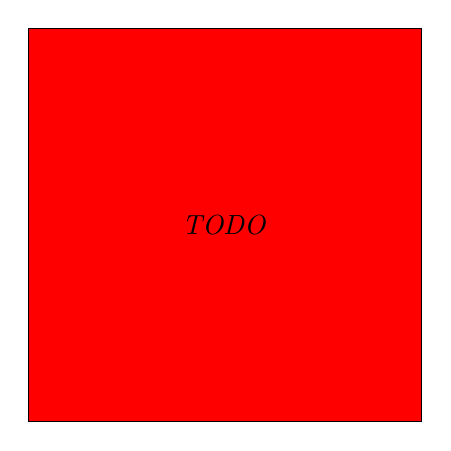
\begin{tikzpicture}
		\filldraw[fill=red] (0,0) rectangle (5,5) node[pos=.5] {\emph{TODO}};
 	\end{tikzpicture}
	\caption{Ortskurve des Frequenzgangs des zeitdiskreten Integrierers}
	\label{fig:6-7}
\end{figure}
Ein Vergleich mit der Frequenzgangortskurve des zeitkontinuierlichen Integrierers zeigt auch hier, dass der zeitdiskrete Integrierer eine Näherung darstellt, deren Fehler nur für kleine \(\omega\) und kleine \(K_I T\) zu tolerieren sind.

Durch die Periodizität der Frequenzgänge zeitdiskreter Übertragungssysteme bekommt die Frequenz
\begin{equation}
	\omega_S = \frac{\pi}{T}
\end{equation}
eine besondere Bedeutung.
Sie wird auch als ``Shannon-Frequenz'' bezeichnet, weil ein von Shannon formuliertes sog. Abtasttheorem besagt, dass eine zeitkontinuierliche Funktion aus ihren Abtastwerten nur dann fehlerfrei rekonstruiert werden kann, wenn die höchste in dieser Funktion enthaltene Frequenz kleiner ist als die Shannon-Frequenz
\begin{equation}
	\omega_{\text{max}} < \omega_S.
\end{equation}
Mit der Periodendauer bzw. der Abtastzeit erhält man
\begin{equation}
	\frac{2\pi}{T_{\text{min}}} < \frac{\pi}{T}
\end{equation}
und daraus die Aussage, dass die Abtastzeit im Sinne des Shannon-Theorems kürzer sein muss als die Hälfte der kürzesten Periodendauer in der abzutastenden Funktion
\begin{equation}
	T < \frac{T_{\text{min}}}{2}.
\end{equation}
\begin{figure}[ht]
	\centering
	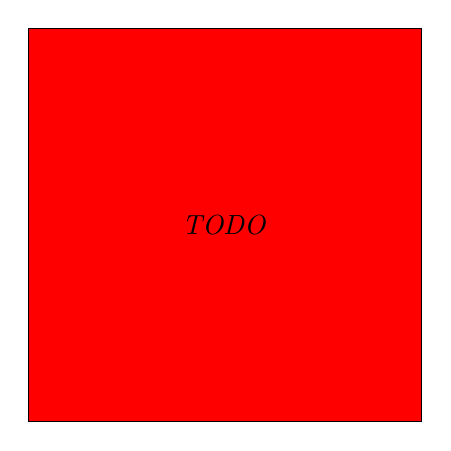
\begin{tikzpicture}
		\filldraw[fill=red] (0,0) rectangle (5,5) node[pos=.5] {\emph{TODO}};
 	\end{tikzpicture}
	\caption{Verfälschung durch Unterabtastung}
	\label{fig:6-8}
\end{figure}
Bild \ref{fig:6-8} zeigt in besonders drastischer Weise die Folgen einer Verletzung des Shannon-Theorems.
Ein sinusförmiges Originalsignal mit einer Frequenz von \(60\sis{\hertz}\) wird mit einer Frequenz von \(50\sis{\hertz}\) abgetastet, obgleich die Abtastfrequenz größer als \(120\sis{\hertz}\) sein müsste.
Die Folge dieser so genannten Unterabtastung ist, dass bei umsichtiger Rekonstruktion des abgetasteten Signals aus den Abtastwerten ein sinusförmiges Signal mit einer Frequenz von \(10\sis{\hertz}\) -- der Differenz zwischen Abtastfrequenz und Frequenz des Originalsignals -- entsteht, ein Ergebnis, dass mit dem Original so gut wie nichts verbindet.
Das Beispiel zeigt auch, dass man durch Unterabtastung nicht nur höherfrequente Signalanteile verliert (den Verlust kann man manchmal in Kauf nehmen) sondern auch Verfälschungen des Signals im -- meist interessierenden -- Bereich niedriger Frequenzen erhält, die man im Allgemeinen nicht durch irgendwelche Nacharbeiten an den Abtastwerten beheben kann.
\begin{figure}[ht]
	\centering
	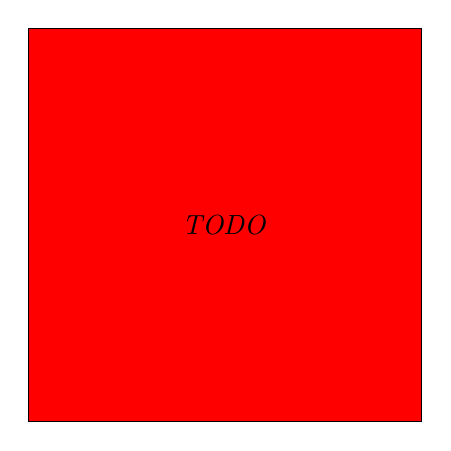
\begin{tikzpicture}
		\filldraw[fill=red] (0,0) rectangle (5,5) node[pos=.5] {\emph{TODO}};
 	\end{tikzpicture}
	\caption{Abtaster mit Anti-Aliasing Filter}
	\label{fig:6-9}
\end{figure}
In der mess- und regelungstechnischen Praxis werden die unerwünschten höherfrequenten Anteile in den abzutastenden zeitkontinuierlichen Funktionen vor dem Abtasten durch ein so genanntes Anti-Aliasing-Filter unterdrückt (Bild \ref{fig:6-9}).
Dieses Filter ist ein zeitkontinuierliches (analoges) Tiefpassfilter, dessen Eckfrequenzen bzw. Durchlassbereich so gewählt sind, dass das Shannon-Theorem sicher erfüllt wird.
Die Bezeichnung des Filters besagt, dass es Verfälschungen der Abtastwerte durch höherfrequente Signalanteile verhindert.
In automatisierten, rechnergestützten Mess- und Datenerfassungseinrichtungen werden die Anti-Aliasing-Filter automatisch an die vom Benutzer eingestellte Abtastfrequenz angepasst.


\subsection{Quasikontinuierliche Abtastregelungen}

Unter quasikontinuierlichen Systemen sollen solche verstanden werden, bei denen im Sinne der Ausführungen am Schluss des Abschnittes 6.1 das Abtastintervall \(T\) so klein ist, dass der Abtastprozess keinen wesentlichen Einfluss auf das Gesamtverhalten hat.
Dies ist i. Allg. dann der Fall, wenn das Abtastintervall deutlich kleiner ist als die Hälfte der Ausgleichzeit \(T_g\) der Regelstrecke (\(T < \frac{T_g}{2}\)) bzw. kleiner als die kleinen Zeitkonstanten der Regelstrecke.
\begin{figure}[ht]
	\centering
	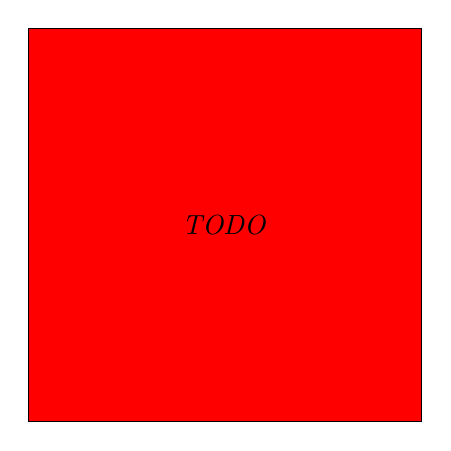
\begin{tikzpicture}
		\filldraw[fill=red] (0,0) rectangle (5,5) node[pos=.5] {\emph{TODO}};
 	\end{tikzpicture}
	\caption{Abtastregelung mit kontinuierlichen Größen}
	\label{fig:6-10}
\end{figure}
Die Mehrzahl der mit einer digitalen Regelung zu versehenden Regelstrecken arbeitet kontinuierlich und kann daher mit den in den Abschnitten 2. bis 4. behandelten Mitteln beschrieben werden.
Das Gesamtsystem soll hier ebenfalls als kontinuierlich arbeitendes System aufgefasst und dargestellt werden.
Dazu geht man von einer Anordnung nach Bild \ref{fig:6-10} aus und definiert für die aus Abtaster, zeitdiskretem Regler und Halteglied bestehende Regeleinrichtung (im Bild mit einer unterbrochenen Linie eingefasst) ein kontinuierliches Ersatzsystem.
Zur Vereinfachung der weiteren Überlegungen wird, wie in Bild \ref{fig:6-11} dargestellt, die Reihenfolge von Regler und Halteglied vertauscht.
Dies entspricht zwar nicht der technischen Wirklichkeit, ist in diesem Fall aber zweckmäßig, weil die so entstehende Reihenschaltung von Abtaster und Halteglied als ein einziges lineares Übertragungsglied aufgefasst und dann durch ein Totzeitglied ersetzt werden kann, das mit einem linearen Regler in Reihe geschaltet ist.
Diese Änderung der Reihenfolge ist auch zulässig, weil Regler und Halteglied lineare Übertragungsglieder sind.
\begin{figure}[ht]
	\centering
	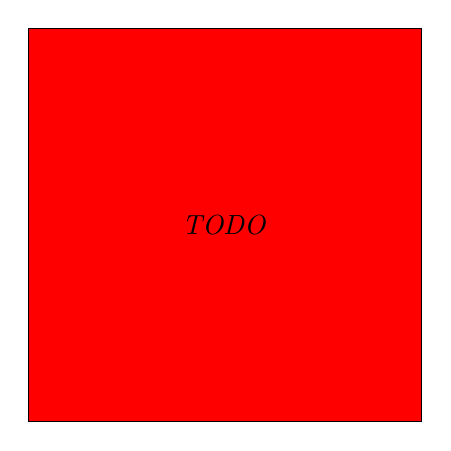
\begin{tikzpicture}
		\filldraw[fill=red] (0,0) rectangle (5,5) node[pos=.5] {\emph{TODO}};
 	\end{tikzpicture}
	\caption{Regeleinrichtung zur Abtastregelung}
	\label{fig:6-11}
\end{figure}
Als Regler werden in der überwiegenden Mehrzahl der Anwendungsfälle Algorithmen eingesetzt, die das Verhalten der in Abschnitt 4.2 eingeführten kontinuierlich wirkenden Regler nachbilden.
Diese Nachbildung ist i. Allg. so gut, dass zur Dimensionierung des Reglers die für kontinuierliche Regler eingeführten Verfahren angewandt werden können.
Die Aufgabe geht dadurch über in die, für den Ersatzregelkreis nach Bild \ref{fig:6-12} einen kontinuierlich wirkenden Regler zu spezifizieren, und diesen dann durch einen geeigneten zeitdiskret wirkenden Algorithmus zu verwirklichen.
\begin{figure}[ht]
	\centering
	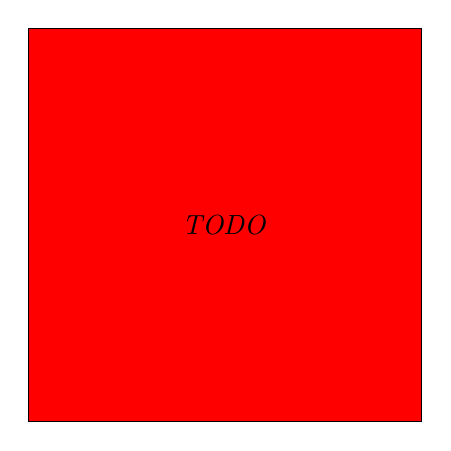
\begin{tikzpicture}
		\filldraw[fill=red] (0,0) rectangle (5,5) node[pos=.5] {\emph{TODO}};
 	\end{tikzpicture}
	\caption{Ersatzregelkreis}
	\label{fig:6-12}
\end{figure}
Der Nachteil der zeitdiskreten Arbeitsweise des Regelalgorithmus wird oft dadurch aufgewogen, dass verschiedene Schwierigkeiten vermieden werden, die die analoge pneumatische oder elektronische Technik enthält und dadurch, dass z.B. keine Einschränkungen im Bereich der realisierbaren Parameterwerte bestehen, wie das bei \(PID\)-Reglern mit einem Verstärker und entsprechender Beschaltung der Fall ist.

Mit der in Abschnitt 6.2 eingeführten Näherung für die Differentiation kann recht einfach die Differenzengleichung gewonnen werden, die einem zeitkontinuierlichen \(PID\)-Regler entspricht.
Aus der Differentialgleichung
\begin{equation}
	y = K_R \parentheses*{u + \frac{1}{T_n}\int_0^t u\d\tau + T_v \dot{u}}
\end{equation}
erhält man durch Ableiten nach der Zeit
\begin{equation}
	\dot{y} = K_R \parentheses*{\dot{u} + \frac{1}{T_n}u + T_v \ddot{u}}.
\end{equation}
Mit Hilfe der entsprechenden Differenzenquotienten -- für die zweite Ableitung ist die Rückwärtsdifferenz zweimal zu bilden -- folgt
\begin{equation}
	\frac{y_k - y_{k - 1}}{T} = K_R \parentheses*{\frac{u_k - u_{k - 1}}{T} + \frac{1}{T_n}u_k + T_v \frac{u_k - 2u_{k - 1} + u_{k - 2}}{T^2}}.
\end{equation}
Geordnet erhält man
\begin{equation}\label{eq:6-38}
	y_k = y_{k - 1} + K_R \parentheses*{\parentheses*{1 + \frac{T}{T_n} + \frac{T_v}{T}}u_k - \parentheses*{1 + 2\frac{T_v}{T}}u_{k - 1} + \frac{T_v}{T}u_{k - 2}}
\end{equation}
als rekursive Rechenvorschrift zur Bestimmung der Werte der Stellgröße eines zeitdiskreten \(PID\)-Reglers.
Man erkennt, dass neben dem aktuellen Wert der Regelabweichung \(u_k\) noch die zu den beiden vorhergehenden Abtastzeitpunkten gehörenden Werte \(u_{k - 1}, u_{k - 2}\) und der vorangehenden Zeitpunkt ermittelte Stellgrößenwert \(y_{k - 1}\) bereitgehalten werden müssen.

Gleichung \eqref{eq:6-38} beschreibt die Wirkungsweise eines sog. Stellungsalgorithmus, der bewirkt, dass dem Halteglied der Wert der Stellgröße selbst zugeführt wird.
Sehr häufig werden zusammen mit digitalen Reglern integrierende Stellglieder eingesetzt, denen dann nur die Änderung der Stellgröße
\begin{equation}\label{eq:6-39}
	\Delta y_k = y_k - y_{k - 1}
\end{equation}
zugeführt werden muss.
Die Gleichungen \eqref{eq:6-38} und \eqref{eq:6-39} ergeben zusammen einen sog. Geschwindigkeitsalgorithmus
\begin{equation}\label{eq:6-40}
	\Delta y_k = K_R \parentheses*{\parentheses*{1 + \frac{T}{T_n} + \frac{T_v}{T}}u_k - \parentheses*{1 + 2\frac{T_v}{T}}u_{k - 1} + \frac{T_v}{T}u_{k - 2}}.
\end{equation}
Als Vorzug integrierender Stellglieder wird im Allgemeinen angesehen, dass sie beim Ausfall des Reglers den zuletzt eingestellten Stellgrößenwert beibehalten.

In Analogie zu den in Abschnitt 5.4 behandelten Einstellregeln für kontinuierliche Regler sind solche Regeln von Takahashi u.a. 1971 für zeitdiskrete Regler veröffentlicht worden.
Zur Beschreibung der Regelstrecke werden entweder Übertragungsfaktor \(K_S\), Verzugszeit \(T_u\) und die Ausgleichszeit \(T_g\) aus einer Sprungantwort benutzt, um die Parameterwerte in Tabelle \ref{tab:6-1} zu bestimmen, oder man stützt sich auf einen Schwingversuch, der den kritischen Reglerübertragungsfaktor \(K_{\text{krit}}\) und die Periodendauer der Schwingung \(T_{\text{krit}}\) liefert, und benutzt Tabelle \ref{tab:6-2}.

Die Reglerparameter sind die eines Geschwindigkeitsalgorithmus von der Form
\begin{equation}
	\Delta y_k = K_P \parentheses*{u_k - u_{k - 1}} + K_I u_k + K_D \parentheses*{u_k - 2u_{k - 1} + u_{k - 2}},
\end{equation}
der mit dem Stellungsalgorithmus in Gleichung \eqref{eq:6-38} und dem Geschwindigkeitsalgorithmus in Gleichung \eqref{eq:6-40} korrespondiert.
Die Tabellen gelten nicht für \(\frac{T_u}{T} \to 0\) und sollten für \(\frac{T_u}{T} < 0,25\) nicht angewandt werden.
Bisher gesammelte Erfahrungen deuten allerdings darauf hin, dass die Einstellwerte für zeitdiskrete Regler nach Tabellen \ref{tab:6-1} und \ref{tab:6-2} weniger allgemein verwendbar sind als die für kontinuierliche nach Tabellen \ref{tab:5-1} und \ref{tab:5-2}.
\begin{table}[ht]
	\centering
	\begin{tabular}{l|ccc}
		\toprule
		Regler & \(K_P\) & \(K_I\) & \(K_D\)\\
		\midrule
		\(P\) & \(\frac{1}{K_S} \cdot \frac{T_g}{T_u + T}\) & \(-\) & \(-\)\\
		\(PI\) & \(\frac{0,9}{K_S} \cdot \frac{T_g}{T_u + 0,5T} - 0,5K_I\) & \(\frac{0,27}{K_S} \cdot \frac{T \cdot T_g}{\parentheses*{T_u + 0,5T}^2}\) & \(-\)\\
		\(PID\) & \(\frac{1,2}{K_S} \cdot \frac{T_g}{T_u + T} - 0,5K_I\) & \(\frac{0,6}{K_S} \cdot \frac{T \cdot T_g}{\parentheses*{T_u + 0,5T}^2}\) & \(\frac{0,5}{K_S} \cdot \frac{T_g}{T}\)\\
		\bottomrule
	\end{tabular}
	\caption{Einstellregeln für zeitdiskrete Regler nach der Sprungantwort der Regelstrecke}
	\label{tab:6-1}
\end{table}
\begin{table}[ht]
	\centering
	\begin{tabular}{l|ccc}
		\toprule
		Regler & \(K_P\) & \(K_I\) & \(K_D\)\\
		\midrule
		\(P\) & \(0,5K_{\text{krit}}\) & \(-\) & \(-\)\\
		\(PI\) & \(0,45K_{\text{krit}} - 0,5K_I\) & \(0,54\frac{K_{\text{krit}}}{T_{\text{krit}}}\) & \(-\)\\
		\(PID\) & \(0,6K_{\text{krit}} - 0,5K_I\) & \(1,2\frac{K_{\text{krit}}}{T_{\text{krit}}}\) & \(0,075K_{\text{krit}} \cdot \frac{T_{\text{krit}}}{T}\)\\
		\bottomrule
	\end{tabular}
	\caption{Einstellregeln für zeitdiskrete Regler nach einem Schwingversuch}
	\label{tab:6-2}
\end{table}
